\paragraph{Learning from Observation (LfO)} \mbox{} \\
\label{sec:lfo}
The goal of \textit{Learning from Observation} is to learn a policy by leveraging \textbf{state-only-demonstration}. This approach has gained attention in recent years because it theoretically allows a robotic system to be programmed as naturally as possible. In fact, in the most promising setting, a robotic system should be able to reproduce a task by observing a human or another robot performing it, without having access to the action performed, as is the case in all the methods described so far. In designing a LfO system there are at least three aspects to consider: \begin{enumerate*}[label=\textbf{(\arabic*)}]
    \item in the case the demonstrator has a different embodiment with respect to the imitator, how can the embodiment mismatch be solved??;
    \item in the case the demonstrator viewpoint differs from the imitator one, how can the correspondence problem between the two different viewpoints be handled?;
    \item once the problems related to the perception subsystem are solved, how is the policy $\pi^{L}$ obtained?. 
\end{enumerate*}
\begin{figure}[htb!]
    \centering
    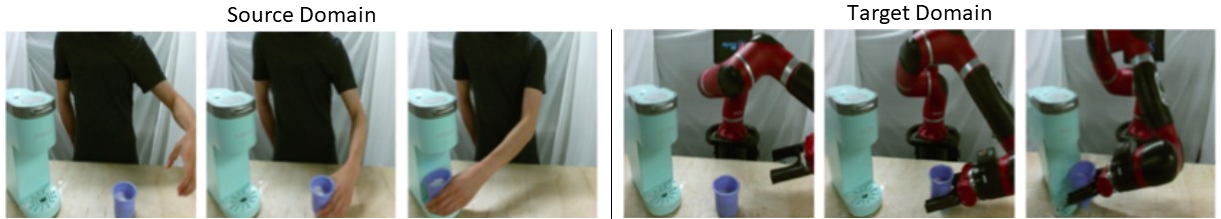
\includegraphics[width=0.9\textwidth]{Figures/images/embodiment_mismatch/embo.png}
    \caption{Representation of embodiment mismatch problem. (Left) The source domain represented by a video of human performing a task. (Right) The target domain, represented by the robot that executes the observed task.}
    \label{fig:embodiment}
\end{figure}


First of all, the points \textbf{(1)} and \textbf{(2)} are going to be answered. Regarding, the embodiment mismatch, this may happen, for example, when the video shows a human performing a task, but the goal is to train a robot (Figure \ref{fig:embodiment}). 
To solve this problem, in \cite{smith2019avid,xiong2021learning_by_watching,li2021meta_watching_video_demonstration}, some sort of image-to-image translation is performed,  while in \cite{zakka2022xirl} the \textit{Temporal-Cycle Consistency} (TCC) \cite{dwibedi2019tcc} was leveraged. In particular, in \cite{smith2019avid,li2021meta_watching_video_demonstration}, the Cycle-GAN \cite{zhu2017cycle_gan} was used to translate image from the source domain (human image) into the corresponding target domain (robot image). The need for an unsupervised image-to-image translation architecture such as the Cycle-GAN arises from the fact that there are not paired images. The network learns two mappings, the first from the source to the target domain $G : X \rightarrow Y$, the second from the target to the source domain $F : Y \rightarrow X$. The dataset for the source domain was composed of human demonstrations as well as a small amount of ``random” data, in which the human moves around the scene but does not specifically attempt the task, while for the target domain, it consists of  robot images executing randomly sampled actions in a few different settings. In \cite{xiong2021learning_by_watching} a similar approach was proposed, but the MUNIT \cite{huang2018munit} architecture was adopted for the image-to-image translation. With respect to the mentioned works, in \cite{zakka2022xirl} a completely different approach has been proposed. Indeed, starting from a set of video demonstrations characterized by both different length and demonstrator embodiment, the TCC approach was used to learn an encoder able to map demonstration frame into the corresponding embodiment-independent embedding. The idea behind TCC was to learn a correspondence between frames of different videos representing the same overall action (Figure \ref{fig:xirl}).
%To do so, for each video $S$ and $T$, of length $N$ and $M$, the frames embedding, $U$ and $V$, are computed. Then one embedding from $U$ is sampled, $u_{i} \in U$, and the nearest neighbor $\tilde{v} = \sum_{j}^M \alpha_{j}v_{j}$ is computed, where $\alpha$ is the result of a soft-max function, at the end the similarity vector $\boldsymbol{\beta}$ is computed between $\tilde{v}$ and each embedding in $U$ by means of a soft-max function. Since $\boldsymbol{\beta}$ is a distribution of probability, assumed to be Gaussian, the whole system is trained by imposing that the peak of $\boldsymbol{\beta}$ must appear at index $i$ (Figure \ref{}.
\begin{figure}[htb]
    \centering
    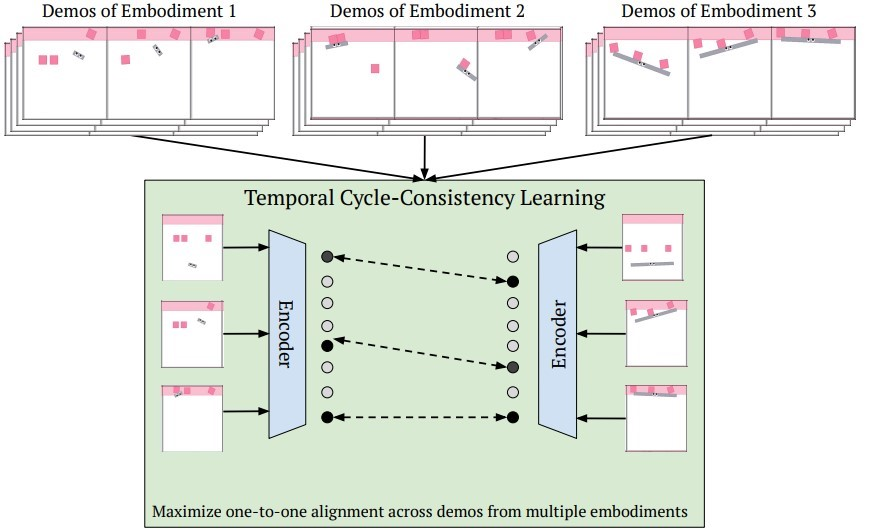
\includegraphics[width=0.65\textwidth]{Figures/images/xirl/xirl.jpg}
    \caption{Temporal-Cycle Consistency representation, used to learn an embodiment-agnostic encoder in \cite{zakka2022xirl}}
    \label{fig:xirl}
\end{figure}

\newline The correspondence problem between different viewpoints was faced by \cite{sermanet2018time_contrastive,liu2018imitation_from_observation}. In \cite{sermanet2018time_contrastive} a CNN was trained by means of a \textit{Triplet-Loss} \cite{schroff2015triplet_loss}. The idea was to train a network able to predict an embedding independent from the view-point, but which contains only task relevant features. To reach this objective the network has to produce an embedding $f(x)$, such that $|| f(x^{a}_{i}) - f(x^{p}_{i})||^{2}_{2} + \alpha < || f(x^{a}_{i}) - f(x^{n}_{i})||^{2}_{2}$ $\forall (f(x^{a}_{i}), f(x^{p}_{i}), f(x^{n}_{i})) \in \mathcal{T}$, where $\mathcal{T}$ is the set of all possible triplets in the dataset. This means that embedding produced by samples coming from different viewpoints, but that share the same time-stamp, $(x^{a}_{i},x^{p}_{i})$, should have a similar embedding, while embedding produced by samples coming from the same viewpoint, but in different time-stamp, $(x^{a}_{i},x^{n}_{i})$, should have a different embedding. In \cite{liu2018imitation_from_observation}, a different approach was used, indeed, a \textit{context translation problem} was solved by means of an Encoder-Decoder architecture (Figure \ref{fig:context-translation}). The proposed architecture was trained on pairs of demonstrations, $\mathcal{D}_{i}=[o^{i}_{0},o^{i}_{1},\dots,o^{i}_{T}]$ and $\mathcal{D}_{j}=[o^{j}_{0},o^{j}_{1},\dots,o^{j}_{T}]$ composed of visual observations. Samples in $D_{i}$ comes from the source context $\omega_{i}$, while samples in $\mathcal{D}_{j}$ comes from the target context $\omega_{j}$. The model must output the observations in $D_{j}$ conditioned on both $\mathcal{D}_{i}$ and the first observation $o^{j}_{0}$ from the target domain. As it will be explained next, the output of both the Time-Contrastive and the Context-Translation network can be used to obtain an engineered reward function.
\begin{figure}[htbp]
    \centering
    \begin{subfigure}[b]{0.45\textwidth}
        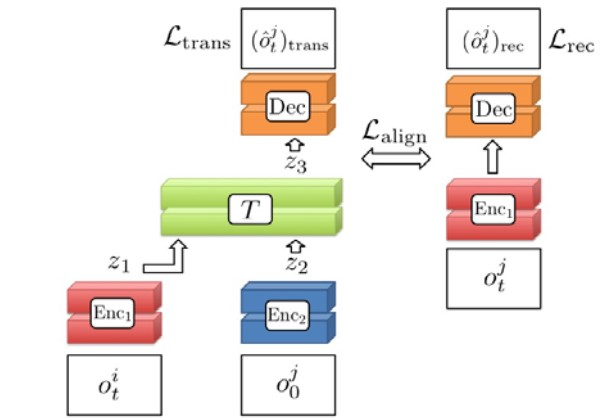
\includegraphics[width=\textwidth]{Figures/images/view_point_mismatch/context-translation-model.jpg}
        \caption{Context-Translation network, proposed in \cite{liu2018imitation_from_observation}}
        \label{fig:context-translation}
    \end{subfigure}
     \hfill
    \begin{subfigure}[b]{0.50\textwidth}
        \centering
        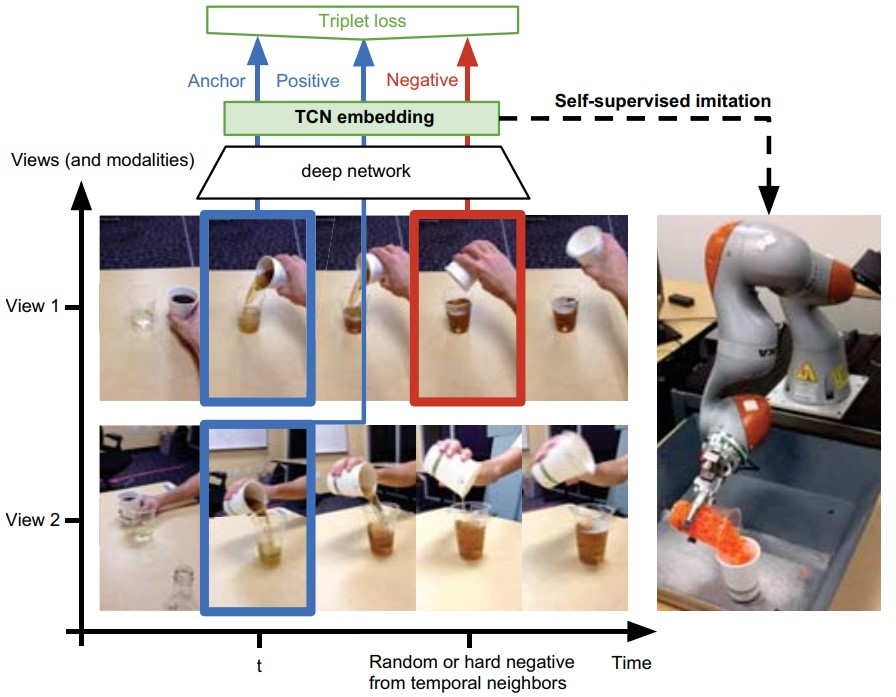
\includegraphics[width=\textwidth]{Figures/images/view_point_mismatch/time-contrastive-network.jpg}
        \caption{Time-Contrastive network, proposed in \cite{sermanet2018time_contrastive}.}
        \label{fig:time_contrastive}
    \end{subfigure}
    \caption{Examples of how the mismatch between demonstrator viewpoint and learner viewpoint can be handled.}
    \label{fig:differet_viewpoint}
\end{figure}


Concerning the way how the policy can be obtained, it is necessary to distinguish between Model-Based and Model-Free methods. 
\newline Among \textbf{Model-Free} methods, a further classification must be made between methods based on \textit{Reward Engineering} or \textit{Adversarial Learning}.
\newline Methods based on Reward Engineering are \cite{sermanet2018time_contrastive,xiong2021learning_by_watching,zakka2022xirl}, in which a hand-designed reward function is used to train a RL agent. In particular, the reward functions obtained in the cited works leverage some sort of \textit{Feature Tracking}. In \cite{sermanet2018time_contrastive} the reward function was $R(o^{l}_{t}) = -||Enc_{1}(o^{l}_{t}) - \frac{1}{n} \sum_{i}^{n}F(o_{t}^{i},o_{0}^{l})||^{2}_{2} - w_{rec} (||o^{l}_{t} - \frac{1}{n} \sum_{i}^{n}M(o_{t}^{i},o_{0}^{l})||^{2}_{2})$. The first term is the classic Feature Tracking reward function, where the goal is to minimize the Euclidian Distance between the encoding of the current learner observation $o^{l}_{t}$ and the encoding of the demonstration in the learner context, the second term has the aim to penalize the policy for experiencing observations that differ from the translated observation.
In \cite{sermanet2018time_contrastive} the reward function was $R(\textbf{v}_{t}, \textbf{w}_{t}) = - \alpha || \ \textbf{w}_{t} - \textbf{v}_{t} \ ||^{2}_{2} - \beta \sqrt{\gamma + || \ \textbf{w}_{t} - \textbf{v}_{t} \ ||^{2}_{2}}$, where $\textbf{v}_{t}$ is the TCN embedding of the video demonstration at timestep t, while $\textbf{w}_{t}$ is the TCN embedding produced by the robot observation (Figure \ref{fig:time_contrastive}).
In \cite{xiong2021learning_by_watching}, first a keypoint-representation is obtained from two consecutive observations, $z_{t}, z_{t+1}$, and from each frame of the translated demonstration video, $z^{E}$. The reward is then computed as $R(z_{t},z_{t+1},z^{E}) = - \lambda_{1} \underset{p}{\min} ||z_{t}-z^{E}_{p}|| - \lambda_{2} \underset{p}{\min} ||(z_{t+1}-z_{t}) - (z^{E}_{p+1}-z^{E}_{p})||$. %(Figure \ref{fig:lbw}). 
In \cite{zakka2022xirl}, the reward function was defined as $R(s_{t}) = -\frac{1}{k} \ || \phi(s_{t}) - g||^{2}_{2}$, where $g$ is the goal embedding, defined as the mean embedding of the last frame of all the demonstration videos in the dataset. Experimental results, on simulation data proved that the proposed method can be used to learn tasks from cross-embodiment demonstrations, outperforming baseline \cite{sermanet2018time_contrastive} in terms of both sample efficiency and performance.%\begin{figure}[htb]
    \centering
    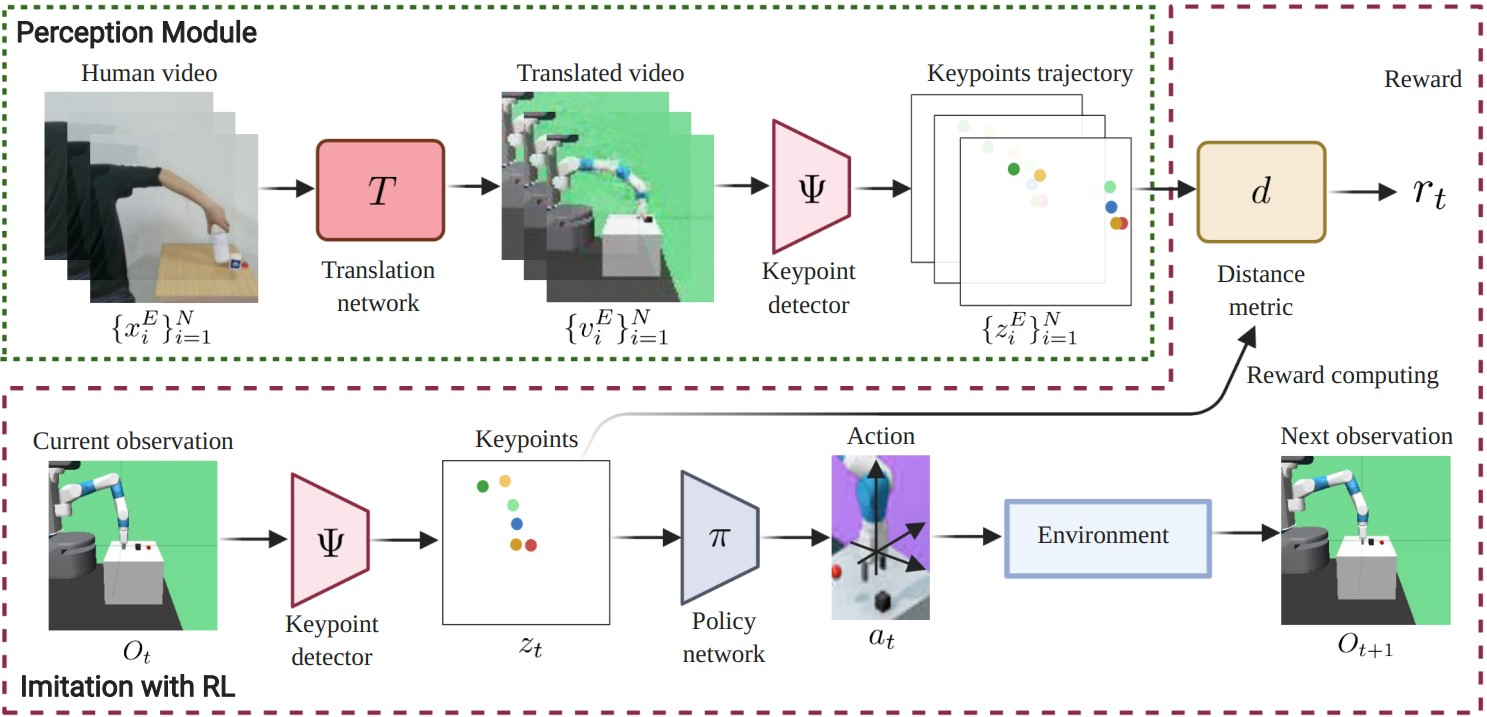
\includegraphics[width=0.7\textwidth]{Figures/images/learning_by_watching/learning_by_watching.jpg}
    \caption{Architecture proposed by \cite{xiong2021learning_by_watching}}
    \label{fig:lbw}
\end{figure}

\newline Regarding the methods based on Adversarial Learning, there are \cite{merel2017learning,torabi2018gaifo}. Obviously, these methods are strictly related to the Generative Adversarial Imitation Learning setting. However, with respect to the methods presented in GAIL paragraph (pag. \pageref{para:gail}), these methods do not assume access to the demonstrator action. Indeed, the goal of the preliminary work \cite{merel2017learning} was to prove that the Adversarial Learning Setting can be effectively used even without the action information. To prove this hypothesis, the authors performed a series of experiments in simulation for a walking task, where the same RL policy was trained in two contexts, the first, where the Discriminator had access to the (state, action) pair, the second where the Discriminator had access to state only demonstrations. The results obtained did not show a substantial difference between the two settings, supporting the hypothesis that in task learning the essential information is contained in the state.
\begin{algorithm}
\caption{GAIfO algorithm \cite{torabi2018gaifo}}
\label{alg:gaifo_algorithm}
\begin{algorithmic}
\Require Initial policy $\pi^{L}_{\phi}$, Initial Discriminator $D_{\theta}$
\Require State-only expert demonstration trajectories $\tau^{E} = \left \{ (s,s') \right \}$
\While {Policy Improves}
    \State Execute $\pi^{L}_{\phi}$ and collect state transitions $\tau^{L} = \left \{ (s,s') \right \}$
    \State Update $D_{\theta}$, with $\mathcal{L}_{D_{\theta}} = - \ ( \ \mathbb{E}_{\tau^{L}}[\log (D_{\theta}(s, s')) ] + \mathbb{E}_{\tau^{E}}[\log(1 - D_{\theta}(s, s'))] \ )$
    \State Update $\pi^{L}_{\phi}$, with reward $ r_{\pi^{L}_{\phi}} = - \ ( \ \mathbb{E}_{\tau^{L}}[\log(D_{\theta}(s, s'))] \ )$
\EndWhile
\end{algorithmic}
\end{algorithm}
\newline The next remarkable work was proposed by the authors of \cite{torabi2018gaifo}, that formalized the \textit{GAIfO} algorithm, (Algorithm \ref{alg:gaifo_algorithm}), that is an extension to state-only demonstration of the GAIL \cite{ho2016gail}. The proposed algorithm was used to train a network to solve tasks in simulation environment \cite{brockman2016openai}, with both low-dimensional state representation, and visual-state representation. Results with respect to the number of demonstrated trajectories are reported in Figure \ref{fig:gaifo_results}.
As it can be noted from the results, GAIfO outperforms previous observation based methods \cite{sermanet2018time_contrastive,torabi2018bco}, in a setting with a low number of expert trajectories. The main drawback of GAIfO is the high number of environmental interactions needed to learn a policy, since the model-free TRPO \cite{schulman2015trpo} algorithm was used to train the policy. This problem was solved by DEALIO \cite{torabi2021dealio}, which replaced the model-free algorithm with PILQR \cite{chebotar2017pilqr} the model-based RL algorithm reported next. \begin{figure}[htbp]
     \centering
     \begin{subfigure}[b]{0.8\textwidth}
        \centering
         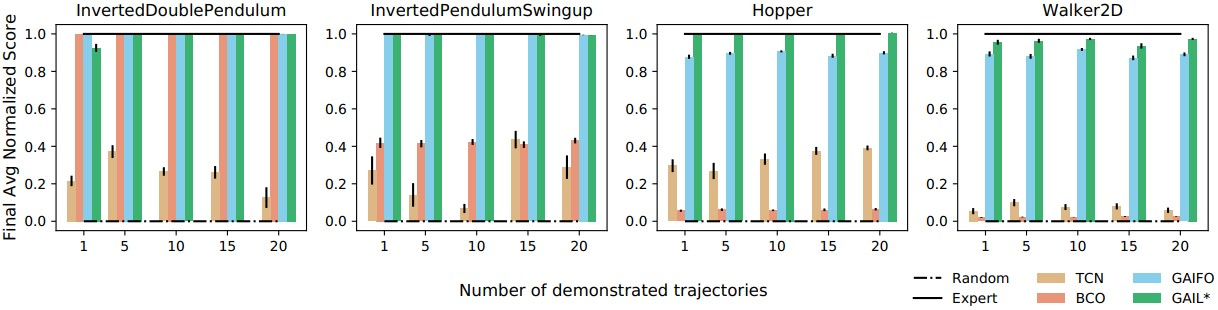
\includegraphics[width=\textwidth]{Figures/images/gaifo_results/gaifo_results.jpg}
         \caption{Experimental results in low-dimensional state space}
         \label{fig:low_dimensional}
     \end{subfigure}

     \begin{subfigure}[b]{0.8\textwidth}
        \centering
         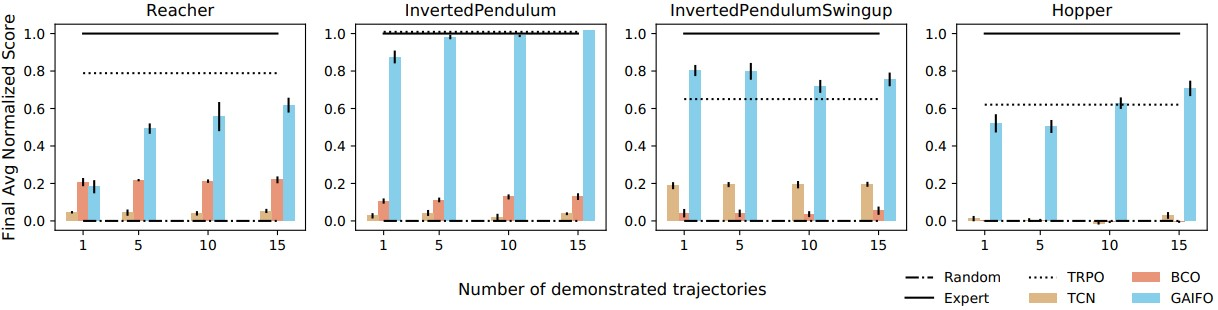
\includegraphics[width=\textwidth]{Figures/images/gaifo_results/gaifo_results_visual.jpg}
         \caption{Experimental results in high-dimensional state space}
         \label{fig:high_dimensional}
     \end{subfigure}
    \hfill
    \caption{Experimental results reported in \cite{torabi2018gaifo}.}
    \label{fig:gaifo_results}
\end{figure}


%result of the Proposition \ref{}, that is an extension to state-only of the Proposition \ref{}, combined with the generative adversarial regularizer in Formula \ref{} characterized by the conjugate in Formula \ref{} 
%\begin{prop}
\label{pre:gaifo_preposition}
$RL\circ  IRLfO_{\psi}$ and $ arg \ min_{\pi^{L} \ \in \ \Pi} \ \psi^{*}(\rho^{s}_{\pi^{L}} - \rho^{s}_{\pi^{E}})$ induce policies that have the same state-transition occupancy measure, $\rho^{s}_{\tilde{\pi}}$
\end{prop}. 
\noindent Among the \textbf{Model-Based} methods a further classification has to be made between methods that obtain the \textit{Inverse Dynamic Model} and methods that obtain the \textit{Forward Dynamic Model}. The former, given in input a transition $(s_{t}, s_{t+1})$, obtain a function $M$, able to map state transition to action i.e., $a_{t} = M(s_{t}, s_{t+1})$. While the latter, given in input a state-action pair $(s_{t}, a_{t})$, aim to learn a function $F$ able to generate the next state $s_{t+1}$, i.e., $s_{t+1} = T(s_{t}, a_{t})$.
\newline Methods that obtain  the Inverse Dynamic Model are \cite{nair2017combining,torabi2018bco,guo2019hybrid_rl,radosavovic2021state_only_demo}. In \cite{nair2017combining} the goal was to obtain a system capable of tying the knot to a rope. To achieve it, a self-supervised learning approach was used to train a CNN, that, taken in input a pair of images $(I_{t}, I_{t+1})$ representing two successive rope states, is able to obtain the action to perform in order to reach the state $I_{t+1}$ from $I_{t}$. To train the CNN, a dataset composed of 30K tuples $(I_{t},a_{t},I_{t+1})$ was collected by means of an exploratory policy. Authors in \cite{torabi2018bco} proposed a general approach, depicted in Figure \ref{fig:bco}, and composed by the two main parts, the learned Inverse Dynamic Model, $M_{\theta}$, and the learned policy $\pi_{\phi}$. In its general form, the learning procedure is an iterative procedure, where the model $M_{\theta}^{i}$ is updated by maximizing the probability $p_{\theta}(a_{t}|s_{t},s_{t+1})$, where the tuples $(s_{t},a_{t},s_{t+1})$ are collected by running the current policy. Once the dynamic model is updated then it is used to infer the action $\tilde{a}_{t}$ given the demonstrations. At the end, since the policy has access to both state and action information, classic BC learning can be run, optimizing the policy parameters through maximum-likelihood estimation $\phi^{*} = \underset{\phi}{argmax} \prod_{i=0}^{N} \pi^{L}_{\phi}(\tilde{a}_{i}|s_{i})$. In \cite{guo2019hybrid_rl}, the same approach as in \cite{torabi2018bco}, but the agent's policy was trained according to a linear combination of Behavioral Cloning and Advantage Actor Critic (A2C) objective function \cite{mnih2016a2c}, i.e., $\mathcal{L}^{hyb}_{\theta} = \mathbb{E}_{s,a}[A(s)\log(a|s;\theta)+\alpha \ \mathcal{H}(\pi^{L}(.|s))] + \mathbb{E}_{(\hat{s}_{t},\hat{s}_{t+1})\sim D}[\log(\pi^{L}(M(\hat{s}_{t},\hat{s}_{t+1})|\theta)]$. The main problem is the assumption to have access to reward function, which can reduce its applicability in real-robot manipulation tasks. In \cite{radosavovic2021state_only_demo}, the work in \cite{Rajeswaran18_learning_complex_dexterous} was extended to state-only demonstration, and the \textit{State-Only Imitation Learning} (SOIL) algorithm was proposed. The context is the one of complex dexterous manipulation, i.e., a simulated humanoid hand must be able to perform tasks such as object reallocation, tool use, in-hand manipulation, and door opening. A neural network was trained to represent the Inverse Dynamic Model, by minimizing the L2-loss, given in input the action performed during the policy rollout. Then, the policy was updated according to \textit{Demo Augmented Policy Gradient} (DAPG) \cite{Rajeswaran18_learning_complex_dexterous}, adapted for state-only demonstration, i.e., $g_{SOIL} = g + \lambda_{0} \ \lambda_{1}^{k} \ \sum_{(s_{t},\tilde{a}_{t} \in D')} \nabla_{\theta}\log\pi^{L}_{\theta}(\tilde{a}_{t},s_{t})$, where $g$ is the Natural Policy Gradient term. The idea is to leverage the demonstrations at the beginning of the training, then exploit the RL algorithm to improve the behavior itself. Indeed, experiments performed in simulation, proved that, with respect to pure RL, the proposed method converges faster, and producing more human-like behaviors.
\begin{figure}[htb]
    \centering
    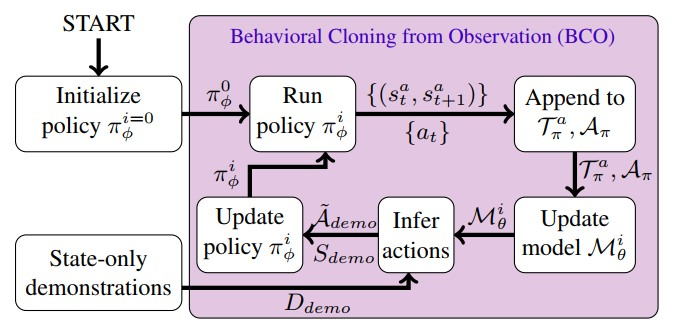
\includegraphics[width=0.6\textwidth]{Figures/images/bco/bco.jpg}
    \caption{Representation of the learning procedure proposed by \cite{torabi2018bco}}
    \label{fig:bco}
\end{figure}

\newline Methods that obtain the Forward Dynamic Model are \cite{smith2019avid,torabi2021dealio}. In \cite{smith2019avid}, once the human video demonstration has been translated into the corresponding robot video, the policy was learned according to the model-based RL algorithm SOLARIS \cite{zhang2019solar}, which allows to obtain a controller optimized according to LQR procedure. The idea was to optimize the policy in a low-dimensional high-regularized \textit{latent space}, generated according to Variational Inference \cite{Kingma2014_vae}. Starting from a sequence of observation-action a Global Dynamic Model over latent trajectory is obtained. Then, given the Latent Dynamic Model, a Linear-Gaussian Controller is obtained through LQR-FLM \cite{levine2014lqr_flm}. Real world robotic experiments, shown that with \textbf{2 hours} of robot interaction it was possible to outperform previous works such as \cite{sermanet2018time_contrastive,torabi2018bco} and classic BC algorithm, on tasks such as ``coffee making" (Figure \ref{fig:embodiment}) and cup-retrieving (i.e., the robot has to take a cup from a closed drawer). 
In \cite{torabi2021dealio} the sample-inefficiency problem of GAIfO \cite{torabi2018gaifo} was addressed. The idea was to exploit the adversarial learning setting with state-only demonstration, which has shown promising results (Figure \ref{fig:gaifo_results}), and combining it with a more data-efficient RL algorithm, such as PILQR \cite{chebotar2017pilqr}. The core of PILQR is the LQR optimization procedure. Generally speaking, it returns a \textit{linear-gaussian controller} (Formula \ref{formula:linear_gaussian_controller}), that optimizes a \textit{quadratic-cost function} (Formula \ref{formula:quadratic_cost_function}), under the assumption of \textit{linear-gaussian dynamic} (Formula \ref{formula:gaussian_dyn}).\begin{equation}
\label{formula:linear_gaussian_controller}
    \pi(a_{t}|s_{t}) = \mathcal{N}(K_{t}s_{t} + k_{t}, S_{t})
\end{equation}

\begin{equation}
\label{formula:quadratic_cost_function}
c(s_{t},a_{t}) = \begin{bmatrix}
s_{t}
\\ 
a_{t}
\end{bmatrix}^{T}C_{t}\begin{bmatrix}
s_{t}
\\ 
a_{t}
\end{bmatrix} + \begin{bmatrix}
s_{t}
\\ 
a_{t}
\end{bmatrix}^{T} c_{t} + cc_{t}
\end{equation}

\begin{equation}
\label{formula:gaussian_dyn}
s_{t+1} \sim P(s_{t+1}|s_{t},a_{t}) = \mathcal{N}(F_{t}
\begin{bmatrix}
s_{t}
\\ 
a_{t}
\end{bmatrix} + f_{t}, \Sigma_{t})
\end{equation}


\noindent In order to use this framework, the linear-gaussian dynamic model was fitted starting from the current policy rollouts, then, to obtain a quadratic cost function as needed by LQR, the dynamic model was used to express the modified discriminator output (Formula \ref{formula:output_discriminator}) as function of the pair $(s_{t},a_{t})$.
\begin{equation}
\label{formula:output_discriminator}
D_{\theta}(s_{t},s_{t+1}) = \frac{1}{2}
\begin{bmatrix}
s_{t}
\\ 
s_{t+1}
\end{bmatrix}^{T}C^{ss}(s_{t},s_{t+1})
\begin{bmatrix}
s_{t}
\\ 
s_{t+1}
\end{bmatrix} + \begin{bmatrix}
s_{t}
\\ 
s_{t+1}
\end{bmatrix}^{T} c^{ss}(s_{t}, s_{t+1})
\end{equation}
Experiments performed in simulation with low-dimensional state space have shown promising results (Figure \ref{fig:dealio_performance}), in terms of sample-efficiency with respect to the GAIfO baseline. However, improvements would be made in order to: \begin{enumerate*}[label=\textbf{(\arabic*)}]
    \item reduce the variance, in order to make the learning process more reliable,
    \item increase the overall performance,
    \item adapt the algorithm to work with real-world robot manipulation tasks.
\end{enumerate*}
\begin{figure}[htbp]
    \centering
    \begin{subfigure}[b]{0.76\textwidth}
        \centering
        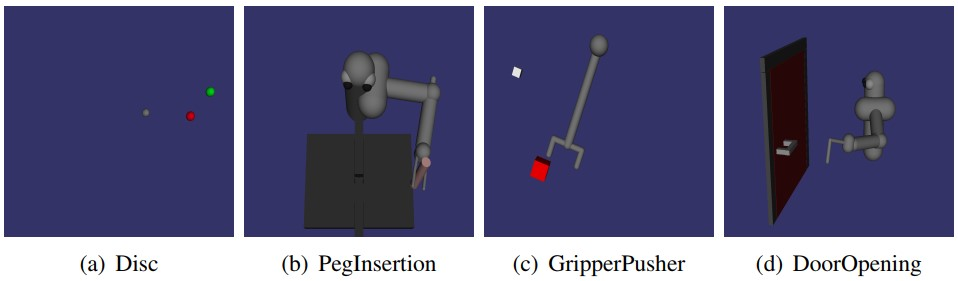
\includegraphics[width=\textwidth]{Figures/images/dealio/dealio_performed_task.jpg}
        \caption{Control Tasks solved in \cite{torabi2021dealio}}
        \label{fig:dealio_task}
    \end{subfigure}
    \hfill
    
    \begin{subfigure}[b]{0.9\textwidth}
        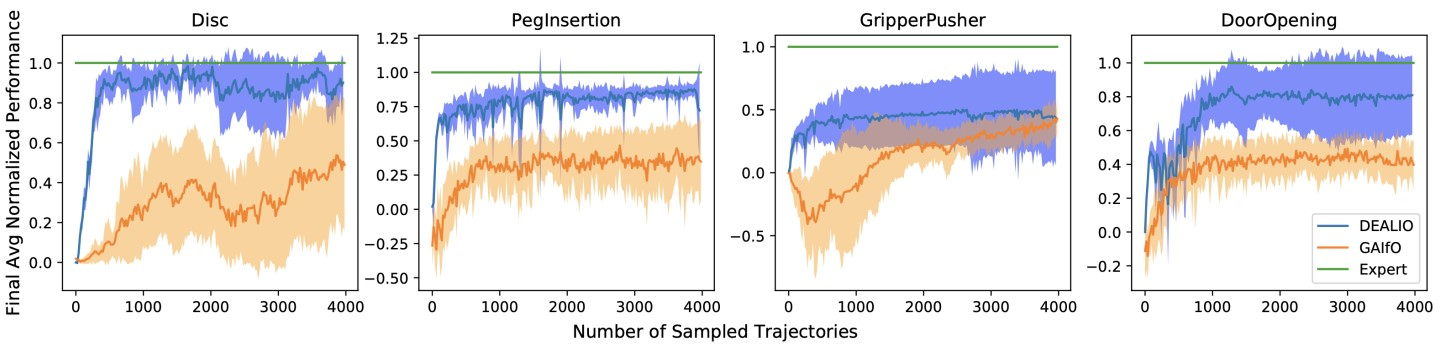
\includegraphics[width=\textwidth]{Figures/images/dealio/dealio_performance.jpg}
        \caption{Performance of DEALIO \cite{torabi2021dealio} compared against GAIfO \cite{torabi2018gaifo}, with respect to the number of trajectories sampled during the learning process.}
        \label{fig:dealio_performance}
    \end{subfigure}
    \caption{DEAILO: (\ref{fig:dealio_task}) Control Tasks, (\ref{fig:dealio_performance}) Performance Level}
    \label{fig:dealio}
\end{figure}


Generally, LfO methods have demonstrated interesting features, such as generating a policy from state-based information alone, supporting the hypothesis that the primary source of information for task learning is the sequence of state transitions. Extrapolating the valuable information to perform actions that induce the desired behavior may not be trivial, mainly if the state space is represented by images of a human operator, leading to the design of architectures composed of different stages, which increase not only the complexity of the system itself but also the amount and diversity of data required for their training. In addition, many methods of interest have been tested in simulated or otherwise relatively simple scenarios, still leaving open the question of whether these methods can be used in real-world complex robotic manipulation tasks.